\documentclass[9pt]{beamer}
\usetheme{Madrid}

% --- TIẾNG VIỆT VỚI PDFLATEX ---
\usepackage[utf8]{inputenc}
\usepackage[T5]{fontenc}
\usepackage[vietnamese]{babel}
\usepackage{comment}
\usepackage[table]{xcolor}
\usepackage{booktabs}
\usepackage{multirow}
\usepackage{amssymb}
% --- GÓI BỔ TRỢ ---
\usepackage{amsmath, amssymb, graphicx, booktabs}
\usepackage{hyperref}
\usepackage{tikz}
\usetikzlibrary{arrows.meta, positioning, shapes.geometric}

% --- GÓI BỔ SUNG CHO CASE STUDIES SLIDES ---
\usepackage[most]{tcolorbox}    % cho codebox, takeaway box
\usepackage{dashrule}           % cho đường kẻ nét đứt thật sự
\usepackage{fancyvrb}           % hỗ trợ verbatim tốt hơn trong tcolorbox

% --- MÀU CHỦ ĐẠO: XANH BIỂN ---
\definecolor{mainblue}{RGB}{0, 100, 180}
\definecolor{darkblue}{RGB}{0, 60, 120}
\definecolor{lightblue}{RGB}{200, 225, 255}
\definecolor{emphred}{RGB}{200, 30, 30}
\definecolor{emphgreen}{RGB}{0, 120, 60}

% --- MÀU BỔ SUNG CHO CODE BLOCKS ---
\definecolor{okGreen}{RGB}{27, 127, 58}
\definecolor{badRed}{RGB}{180, 35, 24}
\definecolor{accentBlue}{RGB}{31, 78, 121}
\definecolor{codeKey}{RGB}{106, 27, 154}
\definecolor{dashGray}{RGB}{136, 136, 136}

\setbeamercolor{palette primary}{bg=mainblue, fg=white}
\setbeamercolor{palette secondary}{bg=darkblue, fg=white}
\setbeamercolor{palette tertiary}{bg=darkblue, fg=white}
\setbeamercolor{palette quaternary}{bg=mainblue, fg=white}
\setbeamercolor{structure}{fg=mainblue}
\setbeamercolor{frametitle}{fg=white, bg=mainblue}
\setbeamercolor{title}{fg=white, bg=mainblue}
\setbeamercolor{block title}{bg=mainblue, fg=white}
\setbeamercolor{block body}{bg=lightblue!40, fg=black}
\setbeamercolor{block title alerted}{bg=red!70, fg=white}
\setbeamercolor{block body alerted}{bg=red!10, fg=black}
\setbeamercolor{block title example}{bg=emphgreen, fg=white}
\setbeamercolor{block body example}{bg=green!8, fg=black}

% ============================================================
%  ĐỊNH NGHĨA HỘP TRÌNH BÀY
% ============================================================

% --- Code box: viền liền màu, nền nhạt ---
\newtcolorbox{codebox}[1]{
  enhanced, breakable, sharp corners, boxrule=0pt,
  leftrule=2.5pt, colframe=#1, colback=#1!5,
  fontupper=\ttfamily\scriptsize,
  left=5pt, right=5pt, top=4pt, bottom=4pt}

% --- Takeaway box: hộp kết luận màu xanh ---
\newtcolorbox{takeaway}{
  enhanced, sharp corners, boxrule=0pt, leftrule=3pt,
  colframe=accentBlue, colback=accentBlue!5,
  left=6pt, right=6pt, top=4pt, bottom=4pt,
  fontupper=\small}

% --- Badges: nhãn SUCCESS / FAILURE ---
\newcommand{\okbadge}[1]{\textcolor{white}{\colorbox{okGreen}{\strut\,\scriptsize\textbf{✓ #1}\,}}}
\newcommand{\badbadge}[1]{\textcolor{white}{\colorbox{badRed}{\strut\,\scriptsize\textbf{✗ #1}\,}}}

% --- Đường kẻ nét đứt phân vùng ---
\newcommand{\dashline}{%
  \vspace{4pt}\noindent%
  \textcolor{dashGray}{\hdashrule{\linewidth}{0.5pt}{2pt}}%
  \vspace{4pt}}

% ============================================================

% --- TIÊU ĐỀ ---
\title[Agentic RAG -- TTHC]{\textbf{Assistant hỏi đáp thủ tục hành chính công Việt Nam ứng dụng Agentic RAG}}

\author[Nhóm SE365]{
    Nguyễn Xuân Phúc, Nguyễn Minh Triết \\[0.4cm]
    \small \textit{Giảng viên hướng dẫn:} \\
    \textbf{TS. Đỗ Trọng Hợp, Nguyễn Ngọc Quí}
}

\institute[UIT]{Trường Đại học Công nghệ Thông tin -- Đại học Quốc gia TP.HCM}
\date{}

% --- FOOTER TÙY CHỈNH ---
\setbeamertemplate{footline}{
  \leavevmode%
  \hbox{%
    \begin{beamercolorbox}[wd=.33\paperwidth,ht=2.25ex,dp=1ex,center]{palette primary}%
      \usebeamerfont{author in head/foot}\insertshortauthor
    \end{beamercolorbox}%
    \begin{beamercolorbox}[wd=.34\paperwidth,ht=2.25ex,dp=1ex,center]{palette secondary}%
      \usebeamerfont{title in head/foot}\insertshorttitle
    \end{beamercolorbox}%
    \begin{beamercolorbox}[wd=.33\paperwidth,ht=2.25ex,dp=1ex,center]{palette primary}%
      \usebeamerfont{date in head/foot}Trang \insertframenumber{} / \inserttotalframenumber
    \end{beamercolorbox}%
  }%
  \vskip0pt%
}

\setbeamertemplate{navigation symbols}{}

% --- KHUNG PHÂN TÁCH PHẦN CHÍNH ---
\AtBeginPart{
  \begin{frame}[plain,c]
    \centering
    {\Large\textcolor{darkblue}{\textbf{PHẦN \insertpartnumber}}}\\[0.6cm]
    \textcolor{mainblue}{\rule{0.4\linewidth}{1.5pt}}\\[0.6cm]
    {\Huge\textcolor{mainblue}{\textbf{\insertpart}}}
  \end{frame}
}

% --- HIỆN MỤC LỤC TRƯỚC MỖI PHẦN ---
\AtBeginSection[]{
  \begin{frame}{Mục lục}
    \tableofcontents[currentsection]
  \end{frame}
}

% ======================================================
\begin{document}

% --- TRANG BÌA ---
\begin{frame}
   \titlepage
\end{frame}

% --- MỤC LỤC TỔNG (liệt kê đủ các phần chính) ---
\begin{frame}{Mục lục}
    \tableofcontents[part=1]
    \tableofcontents[part=2]
    \tableofcontents[part=3]
    \tableofcontents[part=4]
    \tableofcontents[part=5]
\end{frame}

% ======================================================
\part{Giới thiệu}

% ======================================================
\section{Giới thiệu đề tài}
\begin{frame}{Giới thiệu đề tài}
  \begin{itemize}
    \item Thủ tục hành chính công Việt Nam gồm hàng nghìn quy trình, mỗi quy trình có hồ sơ, trình tự, lệ phí, thời hạn và căn cứ pháp lý riêng, lại thường xuyên thay đổi.
    \item Thông tin phân tán và viết bằng văn phong pháp lý, người dân và doanh nghiệp khó tra cứu, dễ nộp sai và thiếu giấy tờ.
    \item Đề tài xây dựng một trợ lý hỏi đáp tiếng Việt cho thủ tục hành chính công theo kiến trúc Agentic RAG, trả lời có căn cứ và luôn dẫn nguồn.
  \end{itemize}
\end{frame}

% ======================================================
\section{Tính ứng dụng}
\begin{frame}{Tính ứng dụng}
  \begin{itemize}
    \item Đối tượng sử dụng: người dân, doanh nghiệp và cán bộ bộ phận một cửa.
    \item Kịch bản: tra cứu hồ sơ, lệ phí và thời hạn bằng ngôn ngữ tự nhiên, hỏi đáp đa lượt và phục vụ liên tục.
    \item Lợi ích: giảm đi lại và nộp sai, mọi câu trả lời đều có dẫn nguồn để kiểm chứng.
    \item Mở rộng được sang các lĩnh vực tra cứu văn bản có cấu trúc tương tự.
  \end{itemize}
\end{frame}

% ======================================================
\section{Tính mới so với các giải pháp hiện tại}
\begin{frame}{Tính mới so với các giải pháp hiện tại}
  \begin{itemize}
    \item So với tra cứu từ khoá trên Cổng Dịch vụ công: hỏi đáp bằng ngôn ngữ tự nhiên và tổng hợp thông tin giữa các thủ tục.
    \item So với mô hình ngôn ngữ lớn dùng trần: có kho tri thức làm căn cứ, giảm ảo giác và luôn dẫn nguồn.
    \item So với RAG tĩnh một lượt: hướng agentic tự đánh giá đã đủ thông tin chưa, tự bổ sung tìm kiếm web khi kho nội bộ thiếu.
    \item Minh bạch: trích dẫn nội dòng kèm tô sáng bằng chứng và hiển thị quá trình suy luận.
  \end{itemize}
\end{frame}

% ======================================================
\part{Dữ liệu}

% ======================================================
\section{Dữ liệu thu thập}
\begin{frame}{Quy trình dữ liệu tổng thể}
  Toàn bộ dữ liệu đi qua một pipeline do nhóm tự xây, chạy liền mạch từ trang web tới vector store qua năm bước:
  \begin{center}
    \includegraphics[width=0.98\linewidth]{figures/pipeline_e2e.png}
  \end{center}
  \begin{itemize}
    \item Crawl tải thủ tục, parse chuẩn hoá thành Markdown, chunk cắt theo mục.
    \item Embedding mã hoá mỗi mẩu thành vector, vector store lưu lại để truy xuất.
  \end{itemize}
\end{frame}

\begin{frame}{Nguồn dữ liệu}
  \begin{columns}[T]
    \begin{column}{0.30\textwidth}
      \centering
      \vspace{0.3cm}
      \includegraphics[width=2.4cm]{figures/favicon_dvc.png}\\[0.35cm]
      {\textbf{\textcolor{darkblue}{Cổng Dịch vụ công\\Quốc gia}}}\\[0.15cm]
      {\small \texttt{dichvucong.gov.vn}}
    \end{column}
    \begin{column}{0.68\textwidth}
      \textbf{\textcolor{mainblue}{Trang chứa gì}}
      \begin{itemize}
        \item Toàn bộ thủ tục hành chính công của cả nước, đủ các cấp từ xã phường tới bộ ngành.
        \item Mỗi thủ tục có trình tự, cách thức nộp, thành phần hồ sơ, phí và lệ phí, căn cứ pháp lý và kết quả.
        \item Phân loại theo lĩnh vực, cơ quan thực hiện và đối tượng áp dụng.
      \end{itemize}
      \vspace{0.2cm}
      \textbf{\textcolor{mainblue}{Tính chính thống}}
      \begin{itemize}
        \item Cổng chính thức của Chính phủ, do Văn phòng Chính phủ vận hành.
        \item Dữ liệu pháp lý, cập nhật theo quyết định công bố thủ tục.
        \item Là nguồn nhà nước duy nhất, bảo đảm độ tin cậy cho chatbot.
      \end{itemize}
    \end{column}
  \end{columns}
\end{frame}

\begin{frame}{Dữ liệu thu thập ở đâu}
  \begin{itemize}
    \item Nguồn duy nhất là Cổng Dịch vụ công Quốc gia tại \texttt{dichvucong.gov.vn} -- kho thủ tục hành chính chính thức của Nhà nước.
    \item Nhóm tự thu thập qua API nội bộ của trang thay vì cào HTML, nên dữ liệu ở dạng JSON có cấu trúc và sạch.
    \item Quy trình hai pha do nhóm tự thiết kế: pha LIST quét toàn bộ danh sách, pha DETAIL tải chi tiết từng thủ tục.
  \end{itemize}
  \vspace{0.1cm}
  \begin{center}
    \includegraphics[width=0.95\linewidth]{figures/crawl_pipeline.png}
  \end{center}
\end{frame}

\begin{frame}{Tổng quan dữ liệu đã thu thập}
  \begin{center}
    \includegraphics[width=0.78\linewidth]{figures/collected_stats.png}
  \end{center}
  \begin{itemize}
    \item Thu thập trọn vẹn \textbf{5.208 thủ tục} trên \textbf{281 lĩnh vực}, không sót và không lỗi.
    \item Mỗi thủ tục là một bản ghi JSON riêng, lưu cục bộ trong repo.
    \item Mỗi bản ghi gồm thông tin chung, trình tự, cách thức nộp, hồ sơ, điều kiện, căn cứ pháp lý và kết quả.
  \end{itemize}
\end{frame}

\begin{frame}{Phân bố dữ liệu}
  Kho thủ tục phủ rộng các cấp hành chính và \textbf{281 lĩnh vực} (top: Hải quan, Hàng hải, Khoa học--công nghệ, Ngân hàng, Thuế), cho thấy tính đại diện nhưng có \emph{đuôi dài}.
  \begin{center}
    \includegraphics[width=0.97\linewidth]{figures/data_distribution.png}
  \end{center}
\end{frame}

\begin{frame}{Ví dụ một thủ tục đã thu thập}
  Thủ tục mã \texttt{1.000016} về quỹ đầu tư khởi nghiệp sáng tạo. Bản ghi JSON có nhiều trường lồng nhau, được biến đổi thành tài liệu Markdown gồm nhãn metadata và các mục chuẩn.
  \begin{center}
    \includegraphics[width=0.96\linewidth]{figures/sample_anatomy.png}
  \end{center}
\end{frame}

% ======================================================
\section{Embedding và cơ sở dữ liệu vector}
\begin{frame}{Embedding}
  \begin{itemize}
    \item Mỗi mẩu văn bản được mã hoá thành vector bằng mô hình \texttt{text-embedding-3-large} của Azure OpenAI, 3072 chiều.
    \item Mô hình đa ngữ, biểu diễn tốt ngữ nghĩa tiếng Việt, thay cho embedding cục bộ.
    \item Corpus được cắt thành \textbf{33.255 mẩu} (trung bình 6,39 mẩu/thủ tục, theo 8 loại mục), embedding một lần rồi lưu lại để tái sử dụng.
  \end{itemize}
  \begin{center}
    \includegraphics[width=0.9\linewidth]{figures/embedding_flow.png}
  \end{center}
\end{frame}

\begin{frame}{Cơ sở dữ liệu vector}
  \begin{itemize}
    \item Vector lưu trong \texttt{ChromaVectorStore}, kèm \texttt{LanceDB} làm docstore và chỉ mục full-text.
    \item Truy xuất hybrid: kết hợp tìm theo ngữ nghĩa và tìm theo từ khoá BM25.
  \end{itemize}
  \begin{center}
    \includegraphics[width=0.92\linewidth]{figures/vectordb_arch.png}
  \end{center}
\end{frame}

% ======================================================
\part{Hệ thống hỏi đáp}

% ======================================================
\section{Từ baseline tới Agentic RAG}
\begin{frame}{Hai luồng hỏi đáp: baseline và agentic}
  \begin{itemize}
    \item Giai đoạn đầu nhóm xây một \textbf{baseline RAG tuyến tính} (một lượt: truy xuất $\rightarrow$ ghép ngữ cảnh $\rightarrow$ sinh trả lời) làm mốc đánh giá.
    \item Hiện engine production là \textbf{Agentic ReAct hai pha}: tác tử tự quyết khi nào tra cứu kho thủ tục, khi nào bổ sung tìm kiếm web, rồi mới tổng hợp.
    \item Cả hai dùng chung tầng dữ liệu, truy xuất lai, cổng độ liên quan và cơ chế trích dẫn; baseline được giữ làm \emph{mốc so sánh}.
  \end{itemize}
  \begin{center}
    \includegraphics[width=0.97\linewidth]{figures/baseline_rag_concept.png}
  \end{center}
\end{frame}

\begin{frame}{Kiến trúc tổng quan}
  \begin{itemize}
    \item Hệ thống gồm ba tầng: giao diện React, tầng API điều phối và module hỏi đáp.
    \item Giao diện và API là lớp vỏ nhận câu hỏi và truyền kết quả về theo dòng sự kiện (SSE).
    \item Phần trình bày sau tập trung vào logic xử lý đầu vào và pipeline bên trong module hỏi đáp.
  \end{itemize}
  \begin{center}
    \includegraphics[width=0.96\linewidth]{figures/baseline_arch.png}
  \end{center}
\end{frame}

% ======================================================
\section{Module hỏi đáp}
\begin{frame}{Năm bước trong module hỏi đáp}
  \begin{itemize}
    \item \textbf{Xử lý đầu vào:} chuẩn hoá câu hỏi thành truy vấn tra cứu đứng vững một mình.
    \item \textbf{Truy xuất lai:} kết hợp tìm theo ngữ nghĩa và tìm theo từ khoá BM25, sau đó khử trùng lặp.
    \item \textbf{Sàng lọc:} chấm điểm liên quan, loại mẩu điểm bằng không.
    \item \textbf{Sinh trả lời:} gói ngữ cảnh còn lại, sinh câu trả lời tiếng Việt có dấu trích dẫn.
    \item \textbf{Trình bày nguồn:} tách nhóm trích dẫn và nhóm tham khảo, kèm sơ đồ tư duy và mức tự tin.
  \end{itemize}
  \begin{center}
    \includegraphics[width=0.95\linewidth]{figures/baseline_pipeline.png}
  \end{center}
\end{frame}

\begin{frame}{Xử lý đầu vào}
  \begin{columns}[T]
    \begin{column}{0.44\textwidth}
      \begin{itemize}
        \item Trước khi truy xuất, module chuẩn hoá câu hỏi để truy vấn tra cứu đứng vững một mình.
        \item Câu dài đã đủ thông tin thì giữ nguyên làm truy vấn.
        \item Câu ngắn thường là câu nối tiếp thiếu ngữ cảnh, module dựa lịch sử hội thoại viết lại thành truy vấn đầy đủ.
        \item Nếu chỉ là chào hỏi xã giao thì bỏ truy xuất, đáp lại tự nhiên qua chỉ dẫn hệ thống.
      \end{itemize}
    \end{column}
    \begin{column}{0.56\textwidth}
      \begin{center}
        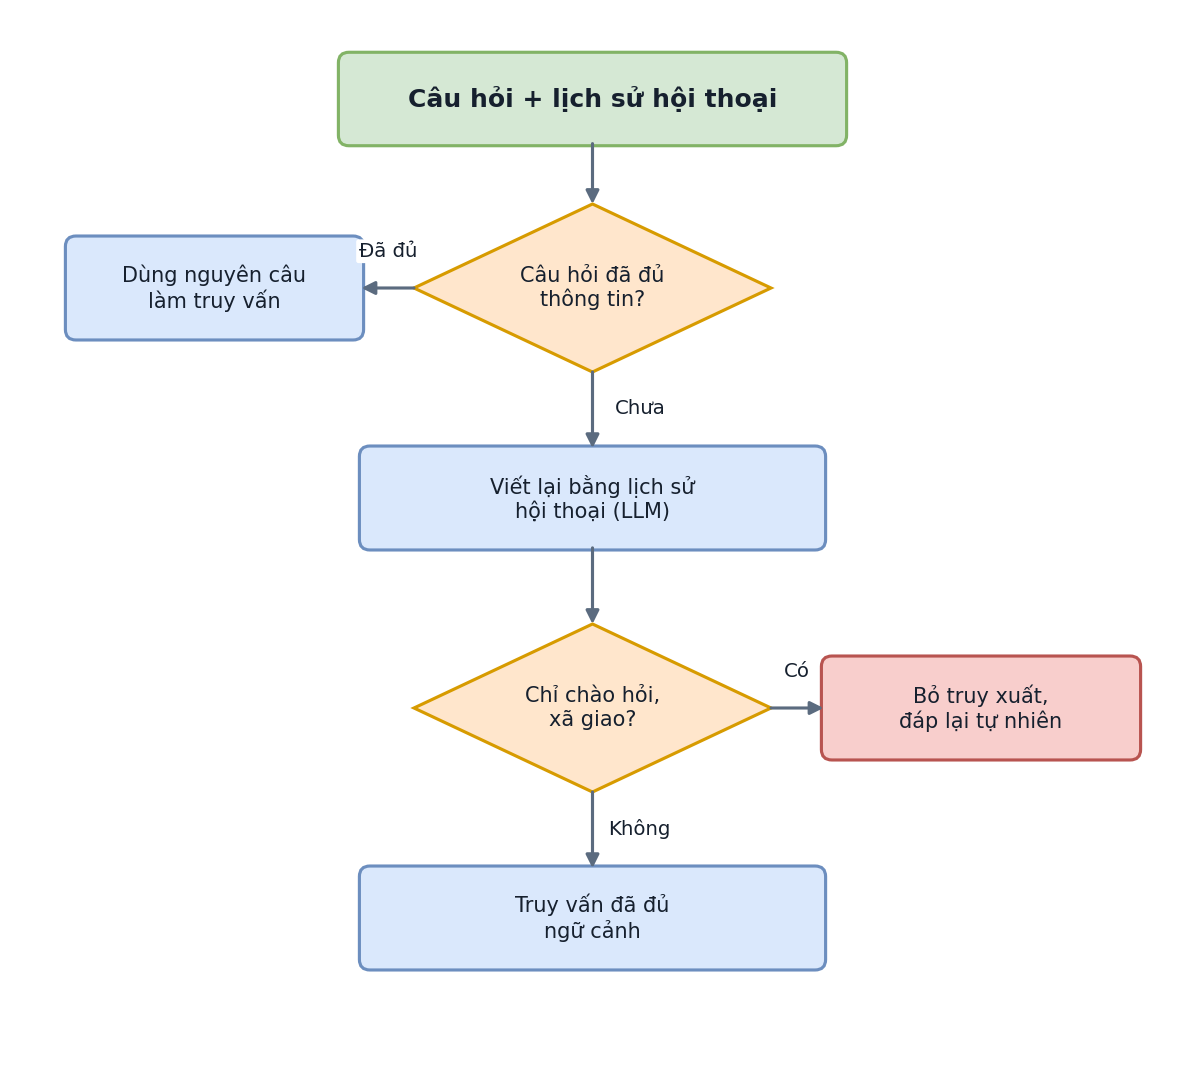
\includegraphics[width=\linewidth]{figures/baseline_input_logic.png}
      \end{center}
    \end{column}
  \end{columns}
\end{frame}

\begin{frame}{Cổng độ liên quan và quyết định từ chối}
  \begin{columns}[T]
    \begin{column}{0.46\textwidth}
      \begin{itemize}
        \item Cơ chế chống mô hình bịa thông tin khi kho không có thủ tục phù hợp (dùng chung cho cả hai engine).
        \item Chấm điểm liên quan đồng bộ ngay trước khi sinh, để mô hình chỉ thấy ngữ cảnh thực sự liên quan.
        \item Nếu mọi mẩu bị chấm điểm bằng không, hệ thống trả câu thông báo ngoài phạm vi cố định và không gọi mô hình sinh.
        \item Quyết định từ chối do mã nguồn kiểm soát theo điểm liên quan, không phó mặc cho mô hình.
      \end{itemize}
    \end{column}
    \begin{column}{0.54\textwidth}
      \begin{center}
        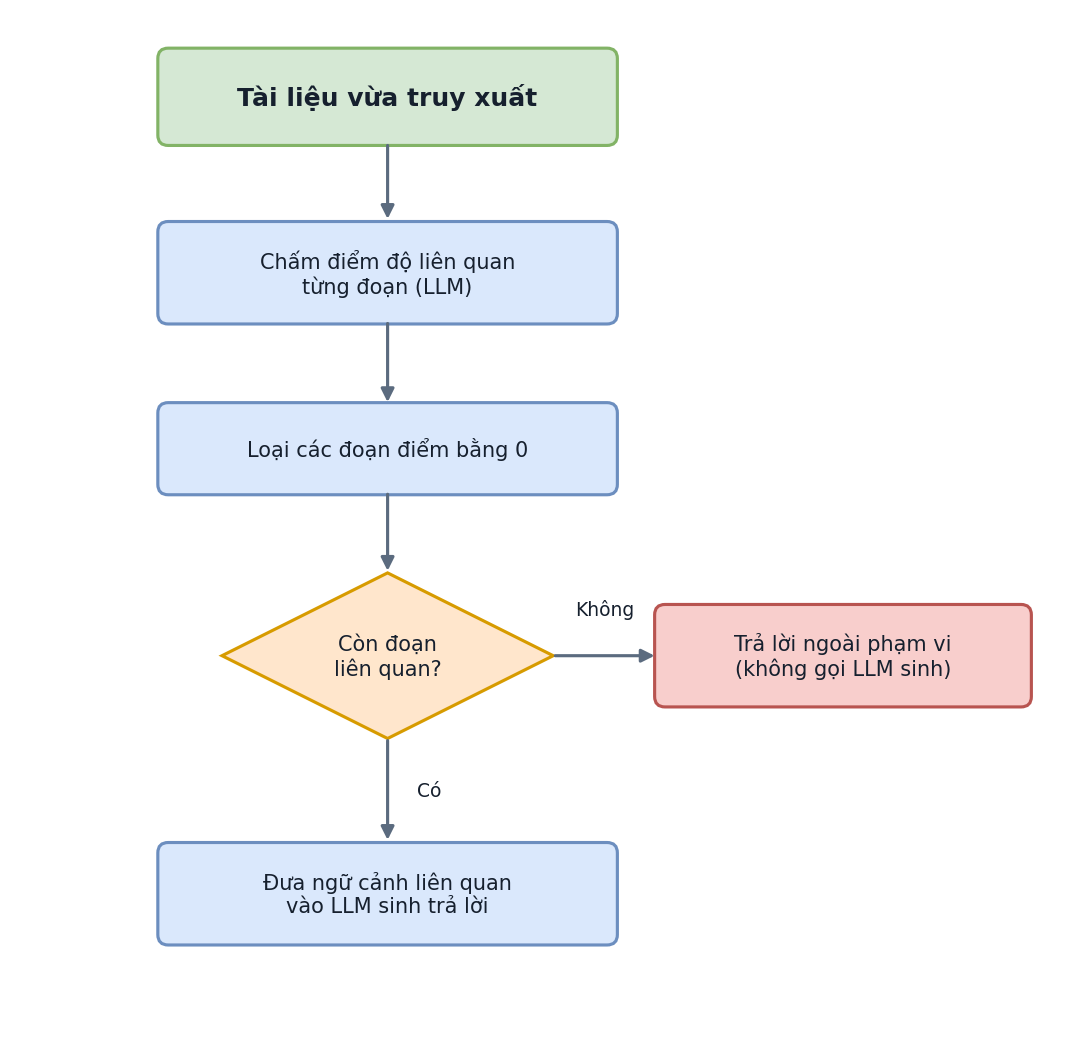
\includegraphics[width=\linewidth]{figures/baseline_relevance_gate.png}
      \end{center}
    \end{column}
  \end{columns}
\end{frame}

% ======================================================
\section{Luồng chính: Agentic ReAct}
\begin{frame}{Luồng chính: Agentic ReAct hai pha}
  \begin{itemize}
    \item \textbf{Pha 1 -- gom nguồn:} tác tử lặp \emph{suy nghĩ $\rightarrow$ hành động $\rightarrow$ quan sát}; ưu tiên tra cứu kho nội bộ, tự đổi truy vấn hoặc tìm web khi nguồn chưa đủ liên quan (Corrective-RAG).
    \item Tách câu hỏi phức thành các câu con và bổ sung ngữ cảnh cho hội thoại đa lượt trước khi truy xuất.
    \item \textbf{Pha 2 -- tổng hợp:} gom nguồn theo từng thủ tục, kéo đủ các mục liên quan, rồi sinh câu trả lời có trích dẫn nội dòng.
    \item Baseline tuyến tính vẫn là mốc so sánh để đo mức cải thiện.
  \end{itemize}
  \begin{center}
    \includegraphics[width=0.9\linewidth]{figures/future_agentic_loop.png}
  \end{center}
\end{frame}

\begin{frame}{Trích dẫn nội dòng và minh bạch}
  \begin{itemize}
    \item Câu trả lời sinh kèm dấu trích dẫn nội dòng, mỗi dấu trỏ về một mẩu tài liệu cụ thể; hệ dò khớp để tô sáng đúng đoạn được trích.
    \item Nguồn tách hai nhóm: nhóm được trích dẫn trực tiếp (có số thứ tự, tô sáng) và nhóm tham khảo; nguồn web được đánh dấu riêng vì chưa thẩm định.
    \item Hiển thị các bước suy luận của tác tử và gợi ý câu hỏi tiếp theo để người dùng kiểm chứng và dẫn dắt hội thoại.
  \end{itemize}
  \begin{center}
    \includegraphics[width=0.84\linewidth]{figures/baseline_citation_flow.png}
  \end{center}
\end{frame}

% ======================================================
\part{Thí nghiệm và Kết quả}

% ======================================================
\section{Thiết kế thí nghiệm}
\begin{frame}{Thiết kế thí nghiệm}
  \begin{itemize}
    \item Hai thí nghiệm độc lập: \textbf{exp01 -- Retrieval} (hệ có tìm đúng tài liệu không, gold = mã thủ tục) và \textbf{exp02 -- Generation \& Citation} (dùng tài liệu trả lời \& trích dẫn có trung thực không, engine ReAct).
    \item \textbf{Bộ Ground Truth 210 câu:} 180 câu tự sinh bằng gpt-4o (phân tầng theo lĩnh vực, 6 nhóm năng lực, chống rò rỉ từ khóa) và 30 câu viết tay (20 câu in-scope + 10 câu ngoài phạm vi).
    \item \textbf{Bám chuẩn học thuật:} sinh truy vấn (InPars/Promptagator); đo retrieval bằng Hit@k, MRR, nDCG (DPR, BEIR); đo generation bằng RAG Triad/RAGAS, citation theo ALCE, abstention theo SQuAD 2.0.
    \item Judge cho exp02 là gpt-4o; các chỉ số đo reference-free (so với chính nguồn và câu hỏi).
  \end{itemize}
\end{frame}

% ======================================================
\section{Kết quả truy xuất (exp01)}
\begin{frame}{Kết quả truy xuất}
  \begin{columns}[T]
    \begin{column}{0.46\textwidth}
      \begin{itemize}
        \item Tổng thể (n=180): \textbf{Hit@5 = 0,922}, Hit@10 = 0,972, \textbf{MRR = 0,775}, nDCG@10 = 0,823 -- đạt cả bốn ngưỡng "tốt".
        \item 66\% thủ tục đúng ở vị trí \#1, 88\% trong top-3, chỉ \textbf{4/180 trượt} top-20.
        \item Điểm yếu ở \textbf{thứ hạng \#1} cho truy vấn ngắn / tình huống (Hit@1 chỉ 0,53--0,60), không phải ở recall.
        \item Hit@5 câu viết tay (0,90) xấp xỉ câu tự sinh, xác nhận bộ GT đáng tin.
      \end{itemize}
    \end{column}
    \begin{column}{0.54\textwidth}
      \begin{center}
        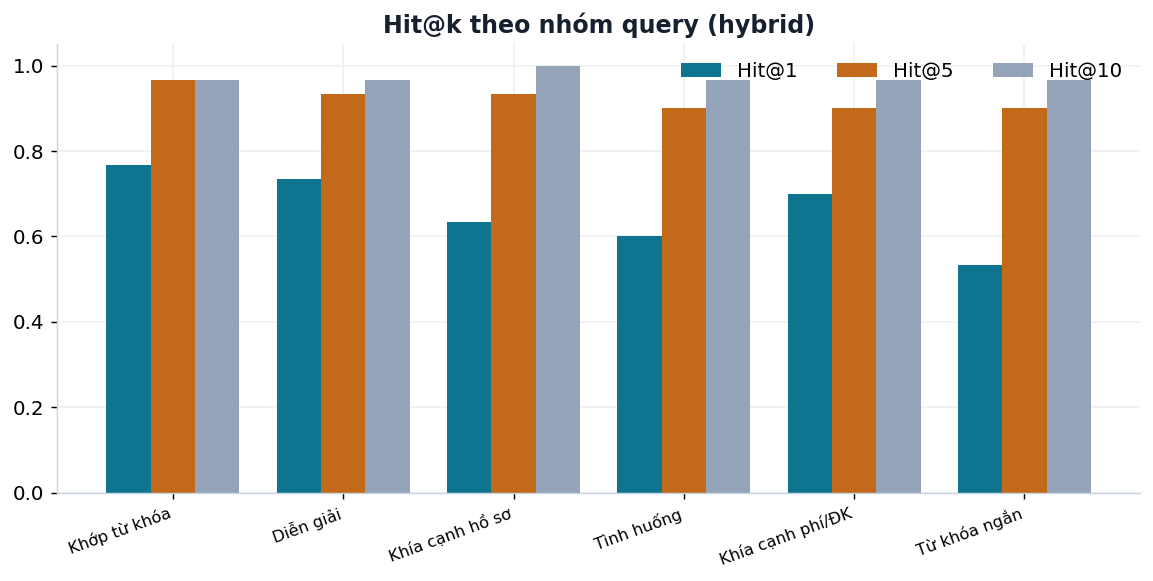
\includegraphics[width=\linewidth]{figures/exp01_hit_by_qtype.png}
      \end{center}
    \end{column}
  \end{columns}
\end{frame}

\begin{frame}{Cổng lọc liên quan và đóng góp của BM25}
  \begin{columns}[T]
    \begin{column}{0.5\textwidth}
      \begin{itemize}
        \item Cổng từ chối câu ngoài phạm vi: \textbf{100\%} (0 tài liệu lọt) -- chặn rác hoàn hảo.
        \item Nhưng chỉ giữ được \textbf{0,65} gold in-scope -- cổng hơi gắt, đôi khi loại nhầm thủ tục đúng.
        \item Điểm yếu này được engine ReAct bù lại ở tầng câu trả lời (xem exp02).
        \item Hybrid xấp xỉ vector-only: \textbf{BM25 đóng góp gần như bằng không} ở top-5 (tokenizer chưa tối ưu tiếng Việt).
      \end{itemize}
    \end{column}
    \begin{column}{0.5\textwidth}
      \begin{center}
        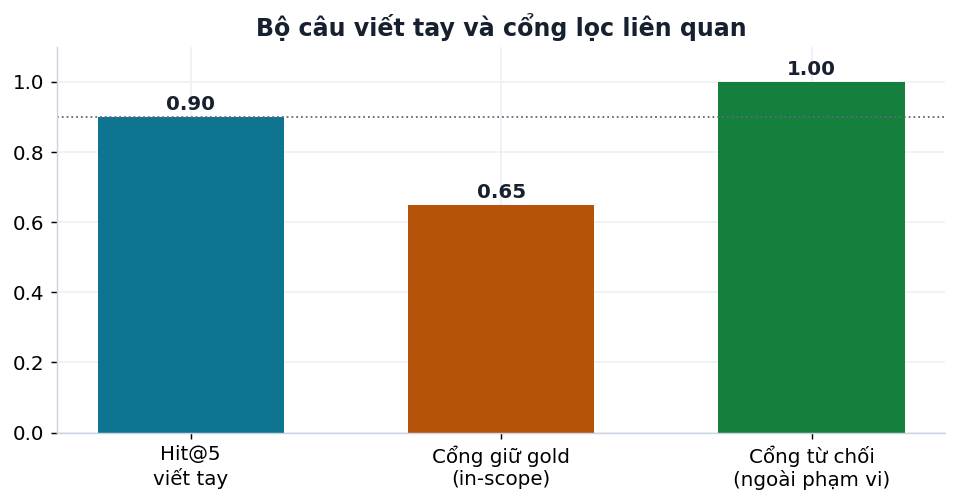
\includegraphics[width=\linewidth]{figures/exp01_gate.png}
      \end{center}
    \end{column}
  \end{columns}
\end{frame}

% ======================================================
\section{Kết quả sinh và trích dẫn (exp02)}
\begin{frame}{Kết quả sinh câu trả lời và trích dẫn}
  \begin{itemize}
    \item \textbf{Faithfulness 0,90} -- câu trả lời bám nguồn, ít bịa (phù hợp domain pháp lý); Answer Relevance 0,75.
    \item \textbf{Citation F1 0,73} -- trích dẫn nội dòng đúng khoảng ba phần tư (recall 0,74 / precision 0,73).
    \item \textbf{Cân bằng từ chối gần lý tưởng:} từ chối 100\% câu ngoài phạm vi mà vẫn trả lời 96\% câu hợp lệ.
  \end{itemize}
  \begin{center}
    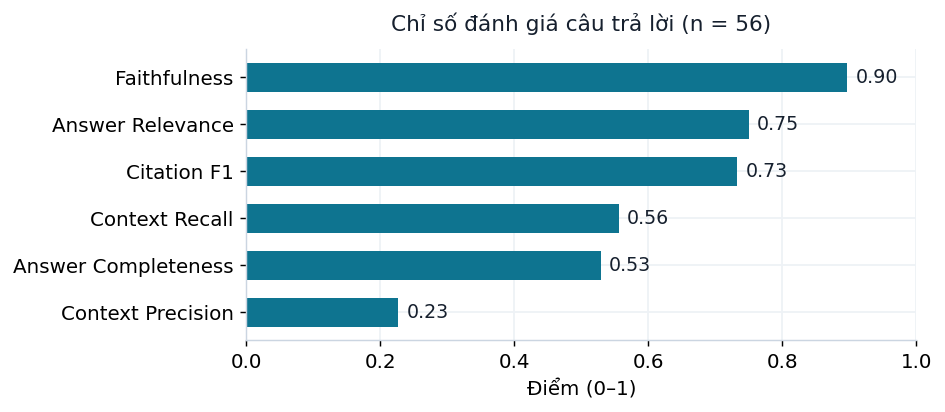
\includegraphics[width=0.76\linewidth]{figures/exp02_metrics.png}
  \end{center}
\end{frame}

\begin{frame}{Giải thích hai chỉ số điểm thấp}
  \begin{itemize}
    \item \textbf{Context Precision 0,23 không phải retrieve rác:} ReAct cố ý kéo đủ mọi mục của thủ tục (trung bình 24,9 đoạn/câu) để trả lời tách bạch -- thiết kế recall-oriented ("thà thừa hơn thiếu").
    \item Bằng chứng đánh đổi có lợi: dù ngữ cảnh "loãng", faithfulness vẫn 0,90 và answer relevance 0,75 -- mô hình lọc đúng phần cần dùng.
    \item \textbf{Completeness 0,53 là cận dưới do cách đo:} ở nhóm hỏi rõ khía cạnh, context recall đạt \textbf{0,84--0,99} và completeness \textbf{0,76--0,89} -- gom đủ và trả lời đủ.
    \item Nhóm câu mơ hồ bị phạt thấp giả vì checklist gold lấy toàn bộ thủ tục trong khi câu chỉ cần một phần.
  \end{itemize}
\end{frame}

% ======================================================
\section{Đối chiếu \& hạn chế}
\begin{frame}{Đối chiếu hai thí nghiệm và hạn chế}
  \begin{itemize}
    \item \textbf{Hai thí nghiệm củng cố lẫn nhau:} điểm yếu chung là câu hỏi mơ hồ / đa ý (tình huống, từ khóa ngắn) -- yếu ở cả Hit@1 lẫn answer relevance, không phải lỗi của riêng tầng nào.
    \item \textbf{ReAct bù cho cổng gắt:} điểm yếu giữ gold 0,65 ở exp01 được kiến trúc hai pha (đổi truy vấn và tìm web) cứu lại -- in-scope answer rate đạt 0,96 ở tầng câu trả lời.
    \item \textbf{Hạn chế:} dùng LLM-judge gpt-4o (hệ sinh cũng gpt-4o) nên có thể thiên lệch tự đánh giá; cỡ mẫu exp02 n=56 (single-run), bộ ngoài phạm vi mới n=8.
    \item Đánh giá reference-free đo "trung thực với nguồn", chưa đo "đúng pháp luật tuyệt đối".
  \end{itemize}
\end{frame}

% ======================================================
\part{Hướng phát triển}

% ======================================================
\section{Việc tiếp theo}
\begin{frame}{Việc tiếp theo}
  \begin{itemize}
    \item \textbf{Hợp thức hóa đánh giá:} spot-check người 20--30 câu để đo đồng thuận judge$\leftrightarrow$người; mở rộng bộ câu ngoài phạm vi.
    \item \textbf{So sánh engine:} chạy cùng bộ metric cho baseline Simple vs ReAct để định lượng mức cải thiện của hướng agentic.
    \item \textbf{Tinh chỉnh cổng độ liên quan:} nới ngưỡng / xét theo cả cụm chunk của thủ tục (đang loại nhầm $\approx$35\% câu in-scope ở tầng retrieval).
    \item \textbf{Cải thiện thứ hạng \#1 \& citation:} reranker mạnh hơn / viết lại truy vấn cho câu ngắn; siết gắn trích dẫn cho câu diễn giải (precision 0,50).
    \item \textbf{Tối ưu thứ cấp:} lọc ngữ cảnh theo khía cạnh câu hỏi để nâng context precision mà không hại completeness.
  \end{itemize}
\end{frame}

% ======================================================
% --- KẾT THÚC ---
\begin{frame}
\begin{center}
\Huge
\textcolor{mainblue}{\textbf{Cảm ơn thầy và các bạn đã lắng nghe}}\\[1cm]
\large \textit{Câu hỏi và Thảo luận}
\end{center}
\end{frame}

\end{document}
